\chapter{Experimentation}
\section{ZMQ-based Handover in srsRAN}
\subsection{Objective}
The first phase aims to understand the basics of S1 handover using srsRAN in a controlled simulation. To emulate the radio layer, we can use ZMQ and GNU radio.

\subsection{Approach}
\begin{itemize}
    \item Following \cite{powell_handover_2021}, I started with a pure simulation-based experiment of inducing an S1 handover
    \item This is accomplished by using ZMQ and GNU Radio to simulate the radio layer.
    \item We set up the experiment by running an Open5gs network core, two srsENBs and a srsUE
    \item The eNBs are connected to the network core over the S1AP interface over TCP on my local machine
    \item The eNBs were both connected to the UE using GNU radio and ZMQ, communicating over various TCP ports.
    \item To emulate propagation loss, we add `multiply` blocks on both connections (send and receive) from UE to each eNB, initially setting it to 1 for the eNB we designate as the source cell and 0 for the "target" cell \todo{insert screenshot of GNU flow graph}
    \item On the srsUE process, we collect the measurement logs, fetching the RSRP for both cells
    \item We gradually increase the multiply for the target cell, until the UE is handed over to the target cell
\end{itemize}

\subsection{Results}
\begin{itemize}
    \item Figure \ref{fig:methods:zmq-s1-handover} shows the results of said experiment
    \item As the handover is triggered by default using the A3 Event Trigger, we can see that the A3 offset used in our configuration was 3dBm.
    \item On a static source analysis of the srsRAN code we see the handover occurs when the following condition is met:
$$\text{RSRP}_\text{Target} - \text{RSRP}_\text{Source} > \text{Hysteresis} + \text{A3 Offset} + \text{Of} + \text{Oc}$$
where 
$$\begin{aligned}\text{Of} &= \text{Frequency Offset}_\text{Target} - \text{Frequency Offset}_\text{Source} \\
\text{Oc} &= \text{Cell Offset}_\text{Target} - \text{Cell Offset}_\text{Source}\end{aligned}$$
for the default setup, $\text{Of}=0$ and $\text{Oc}=0$
\item Furthermore, Hysteresis is set to 0, and in our configuration, A3 Offset was set to 3dBm, so we see srsRAN behaving as expected according to the LTE specification.
\end{itemize}
\begin{figure}
    \centering
    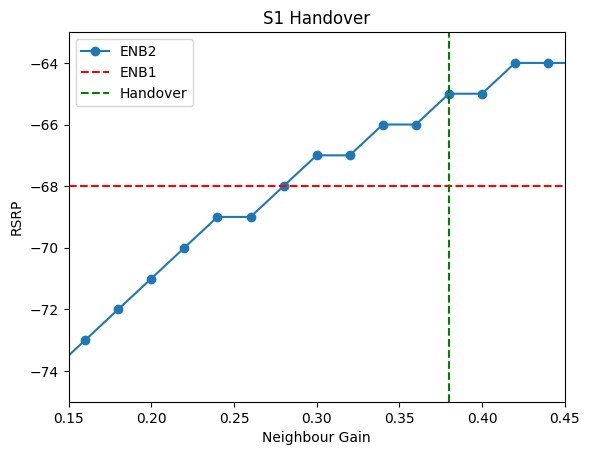
\includegraphics[width=1\linewidth]{src/img/zmq_s1_handover.png}
    \caption{S1 Handover occurring in srsRAN with simulated UE over ZMQ/GNU Radio}
    \label{fig:methods:zmq-s1-handover}
\end{figure}
\subsection{Immediate Discussion}
This phase confirmed srsRAN's adherence to the LTE standard, and a handover was successfully performed in a simulated environment. This phase was limited by the simplistic nature of the simulated radio network, as constants purely dictated network strength. The limited nature of the simulated environment prompted questions about how handovers would occur in more complex environments.

\section{Custom Network Simulator for Large Scale Handovers}
\subsection{Objective}
Building on the initial findings, this phase was focused on understanding the ping-pong metric and the associated triggers, employing a custom large-scale simulator for analysis.

\subsection{Approach}
Inspired by \citep{hatipoglu_handover-based_2020} we reconstructed their non-disclosed tool to simulate large-scale handovers.
\begin{itemize}
    \item We look at  to better understand how large-scale handovers are conducted
    \item We replicate their findings, to understand what causes ping pong
    \item Propagation loss was modelled with path shadow loss (insert equations here)
    \item UE movement is simulated using a random walk with various speed categories
    \item As the authors did not release the tool they built, we reconstructed the tool, as seen in Figure \ref{fig:methods:grouped-uesim}
\end{itemize}
\begin{figure}
    \centering
    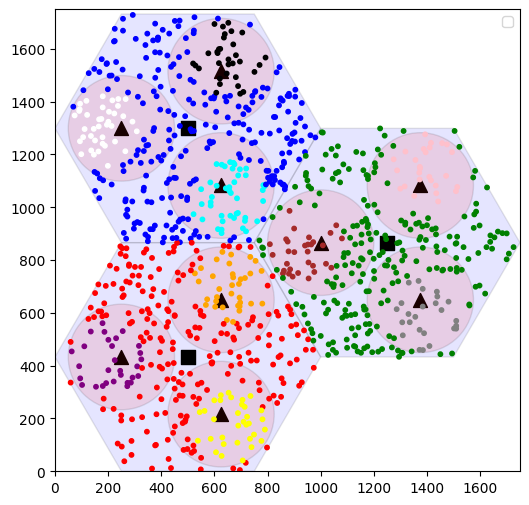
\includegraphics[width=0.75\linewidth]{src//img/grouped_uesim.png}
    \caption{An overview of the 2D simulator}
    \label{fig:methods:grouped-uesim}
\end{figure}
\subsection{Results}
We run the experiment with various handover parameters in Figure \ref{fig:methods:pingpong-uesim}. The impact of the hysteresis value becomes apparent \todo{redo graph showing z-axis}
\begin{figure}
    \centering
    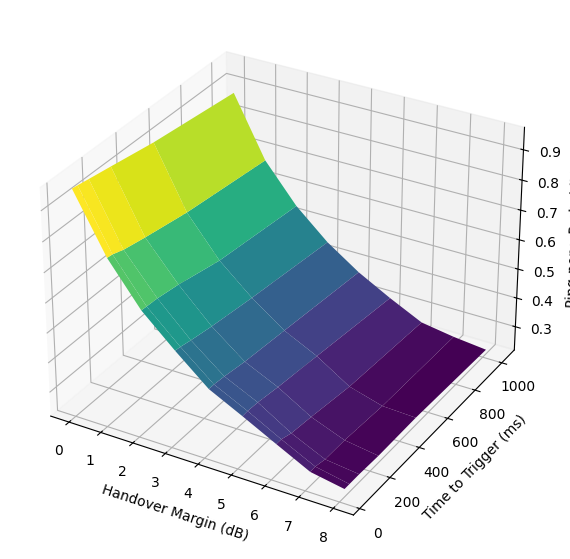
\includegraphics[width=0.5\linewidth]{src//img/pingpong_uesim.png}
    \caption{Ping Pong vs Hysteresis and TTT}
    \label{fig:methods:pingpong-uesim}
\end{figure}
\subsection{Immediate Discussion}
The simulator offered some insights into the conditions which cause ping-pong handovers, however, this was majorly limited by the basic nature of the loss propagation function, as well as highly approximate human movement. This once again reiterates the need for real-world testing to validate these findings \todo{do we validate?}, leading to our next phase of experimentation

\section{Real-world Network Testbed Implementation}
\subsection{Objective}
After performing the initial experiments in a simulator, we move on to testing in the real world to validate our simulation insights and provide real insight into indoor scenarios, utilising a network of radio-enabled srsENBs to examine handover behaviour in a physical environment.
\subsection{Approach}
\begin{itemize}
    \item The testbed consists of 4 NUCs, each connected to an Ettus Research B210 USRP. 
    \item Each NUC runs a modified srsENB process, enabled with an E2 RIC interface to be oRAN compatible. 
    \item Open5gs is running on another server and is connected using the S1 interface
    \item The entire setup is orchestrated using KOperators \todo{find citation}, a Kubernetes deployment framework for ORAN.
    \item We enable two of the eNBs, and run srsUE on an external machine also attached with a B210 USRP
    \item The logs of the UE are saved to disk, with RRC logs set to DEBUG
\end{itemize}
\subsection{Results}
The real-world experiments and the description of the experiment are set out in Figure \ref{fig:methods:real-world-testbed}.
\subsection{Immediate Discussion}
These findings underscored the complexity of indoor scenarios.

Figure \ref{fig:methods:2024-02-09-multi-ho} performs handovers as a UE moves closer and further from a target cell as expected, however, the large noise spikes were not accounted for in the expectations of the experiment. The following experiment in Figure \ref{fig:methods:2024-02-09-rotate} seeks to highlight this possible disparity by rotating the UE back and forth, causing large disturbances to RSRP. 
\begin{figure}[p]
    \centering
    \caption{Real-world Network Testbed Implementation: A series of experiments illustrating various aspects of handover behaviour in a real-world setup.}
    \label{fig:methods:real-world-testbed}
    \begin{minipage}{0.45\textwidth}
    \begin{subfigure}{.9\linewidth}
        \centering
        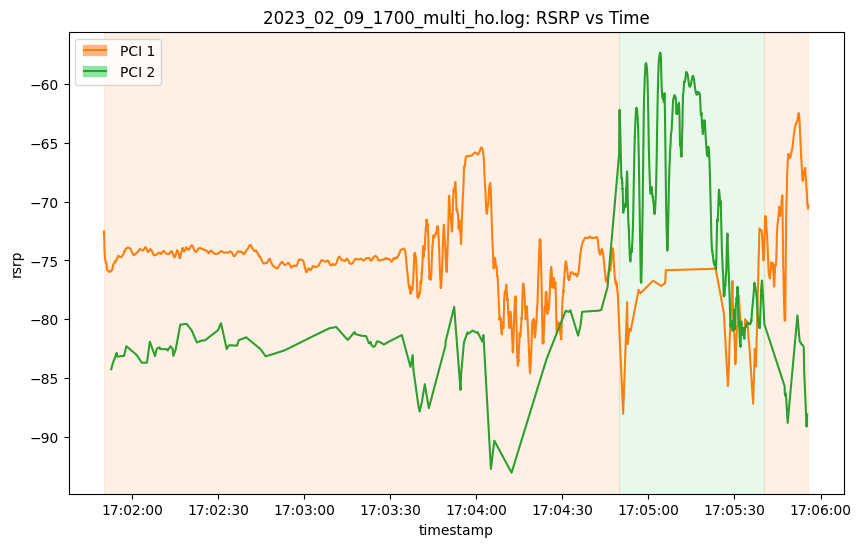
\includegraphics[width=0.9\linewidth]{src//img/2024_02_09_multiho.png}
        \caption{Walking back and forth}
        \label{fig:methods:2024-02-09-multi-ho}
    \end{subfigure}
    \end{minipage}%
    \begin{minipage}{0.45\textwidth}
        \small{Figure \ref{fig:methods:2024-02-09-multi-ho}: Demonstrates the RSRP and connected cell for a walking back and forth episode. This experiment showcases the dynamic RSRP changes as the UE moves closer or further from each eNB.}
    \end{minipage}
    
    \vspace{1cm}
    \begin{minipage}{0.45\textwidth}
    \begin{subfigure}{\linewidth}
        \centering
        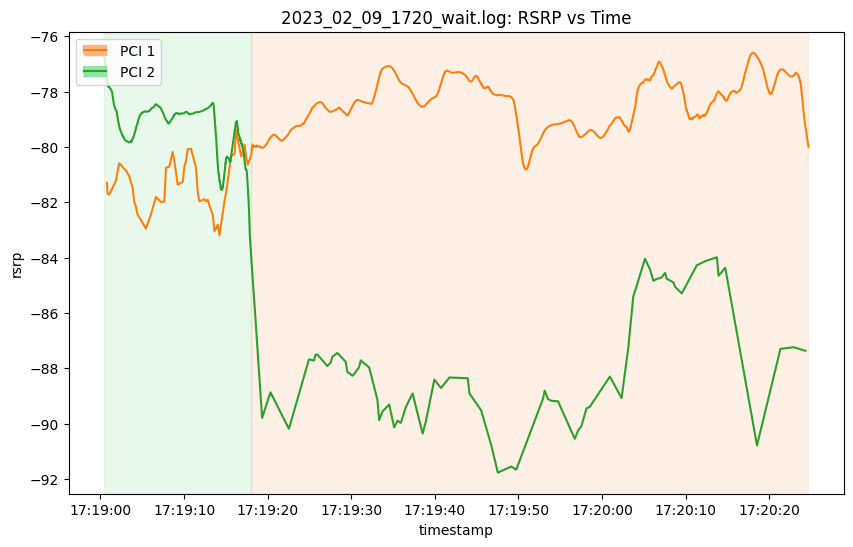
\includegraphics[width=0.9\linewidth]{src//img/2024_02_09_wait.png}
        \caption{2 eNB, no movement}
        \label{fig:methods:2024-02-09-wait}
    \end{subfigure}
    \end{minipage}
    \begin{minipage}{0.45\textwidth}
        \small{Figure \ref{fig:methods:2024-02-09-wait}: Shows the effect of no movement on RSRP measurements, indicating the presence of environmental noise and its potential impact on handover decisions.}
    \end{minipage}
    
    \vspace{1cm}
    \begin{minipage}{0.45\textwidth}
    \begin{subfigure}{\linewidth}
        \centering
        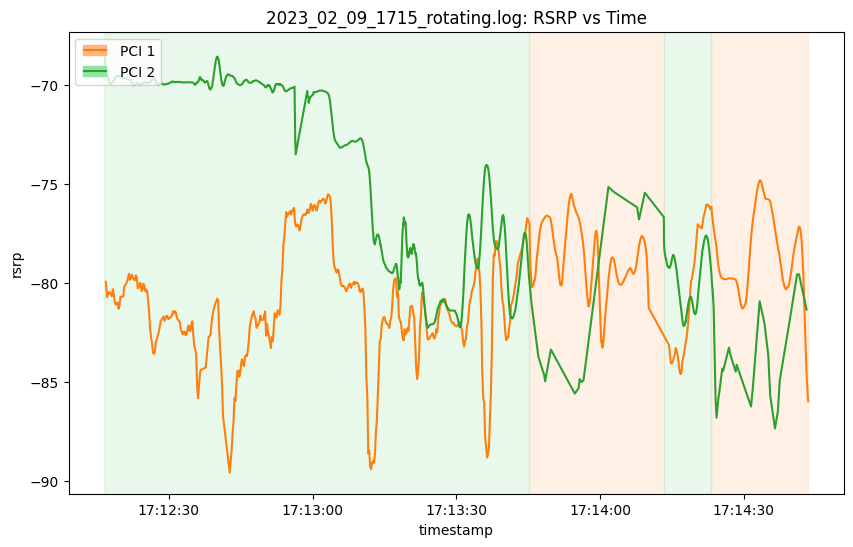
\includegraphics[width=0.9\linewidth]{src//img/2024_02_09_rotating.png}
        \caption{Rotating UE}
        \label{fig:methods:2024-02-09-rotate}
    \end{subfigure}
    \end{minipage}
    \begin{minipage}{0.45\textwidth}
        \small{Figure \ref{fig:methods:2024-02-09-rotate}: Illustrates the impact of rotating the UE on RSRP fluctuations and handover events, highlighting the sensitivity of handover mechanisms to device orientation.}
    \end{minipage}
    
    \vspace{1cm}
    \begin{minipage}{0.45\textwidth}
    \begin{subfigure}{\linewidth}
        \centering
        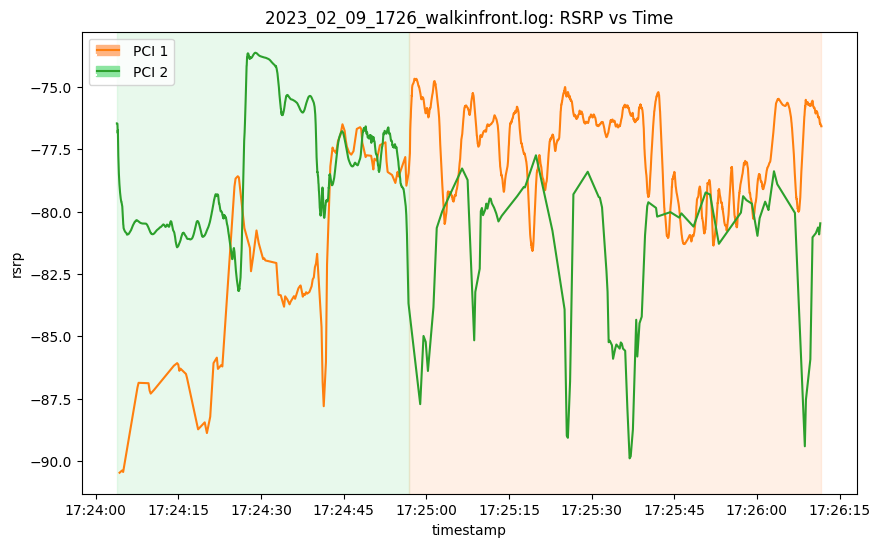
\includegraphics[width=0.9\linewidth]{src//img/2024_02_09_los_block.png}
        \caption{LOS Blockage by walking around}
        \label{fig:methods:2024-02-09-walking}
    \end{subfigure}
    \end{minipage}
    \begin{minipage}{0.45\textwidth}
        \small{Figure \ref{fig:methods:2024-02-09-walking}: Examines the effects of line-of-sight (LOS) blockage by simulating movement around the UE. This scenario reflects real-world dynamics where human movement can influence signal quality and handover behaviour.}
    \end{minipage}
\end{figure}

\clearpage
\section{Handover Impact}
\subsection{Objective}
To understand the impact a handover has on both the network and the UE, we must examine the extent to which a handover impacts throughput and latency
\subsection{Approach}
\begin{itemize}
    \item To determine the actual impact of a handover, we must measure it quantitatively
    \item We run a ping flood from the UE to the EPC, and capture the packets using `tcpdump`
    \item Similarly to the previous experiment, we walk from one eNB to another to induce handover
    \item The packet traces are then analysed with Wireshark to see the latency of each packet. We perform a rolling max smoothing with a window size of 2ms.
    \end{itemize}
\subsection{Results}
    The results are shown in Figure \ref{fig:methods:ping-handover}
\begin{figure}
    \centering
    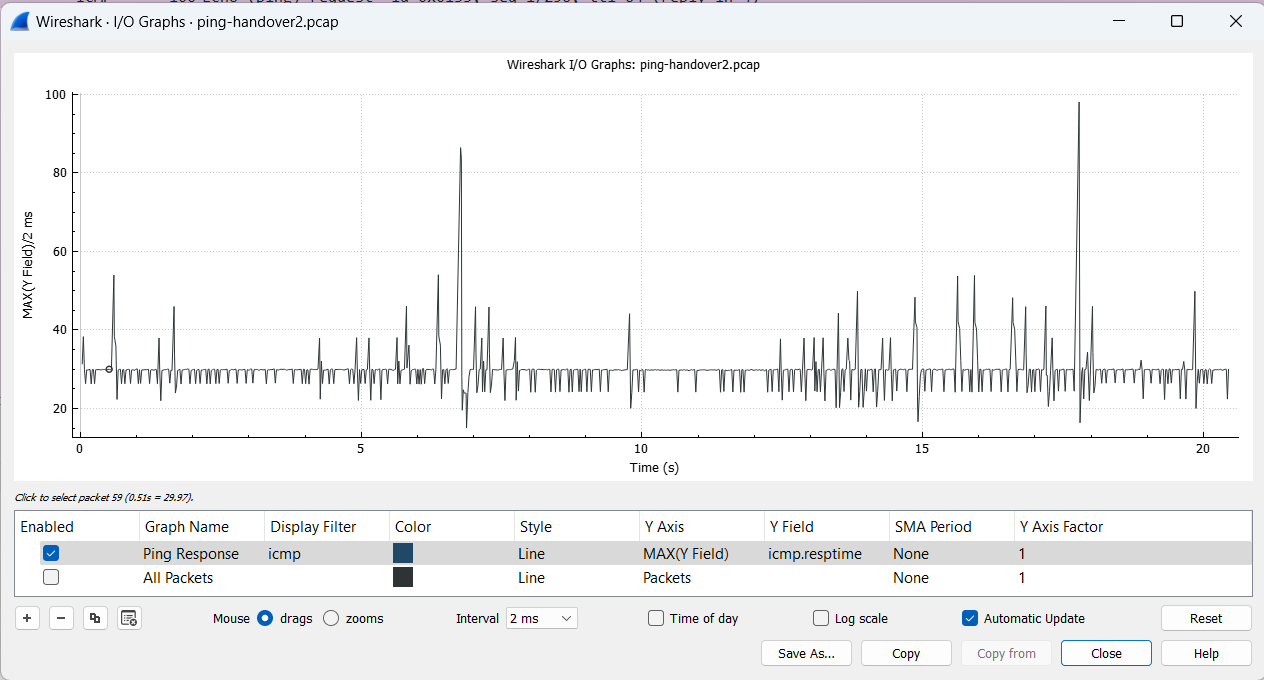
\includegraphics[width=0.75\linewidth]{src//img/ping-handover.png}
    \caption{Wireshark view of Ping during a handover event}
    \label{fig:methods:ping-handover}
\end{figure}
We see a large latency spike during the handover event, however no packets are dropped due to the EPC/eNB buffering any packets received during HO. \todo{explain soft/hard handover} 

\section{High eNB density}
\subsection{Objective}
\begin{itemize}
    \item Repeat the previous experiment but with 4 eNB enabled
    \item Aim to see the extent to which previous findings are heightened or mitigated
    \item Hypothesis: The number of handovers will be much larger
\end{itemize}
\subsection{Approach}
\todo{Run experiment}
\subsection{Results}
\subsection{Immediate Discussion}

\section{Hysteresis Impact}
\subsection{Objective}
\begin{itemize}
    \item Determine how much tuning the hysteresis/A3 threshold value will impact the number of unneeded handovers \todo{Define what an unneeded handover is, possible CQI?}
\end{itemize}
\subsection{Approach}
\todo{Run Experiment}
\subsection{Results}
\subsection{Immediate Discussion}

\section{An Alternative Algorithm}
\subsection{Objective}
\begin{itemize}
    \item Try and build an alternative handover strategy that can mitigate these previous issues, possibly based on CQI
\end{itemize}
\subsection{Approach}
\todo{Run experiment}
\subsection{Results}
\subsection{Immediate Discussion}